%%%%%%%%%%%%%%%%%%%%%%%%%%%%%%%%%%%%%%%%%%%%%%%%%%%%%%%%%%%%%%%%%%%%
%% I, the copyright holder of this work, release this work into the
%% public domain. This applies worldwide. In some countries this may
%% not be legally possible; if so: I grant anyone the right to use
%% this work for any purpose, without any conditions, unless such
%% conditions are required by law.
%%%%%%%%%%%%%%%%%%%%%%%%%%%%%%%%%%%%%%%%%%%%%%%%%%%%%%%%%%%%%%%%%%%%

\documentclass{beamer}
\usetheme[university=bs,faculty=standard]{fibeamer}
\usepackage[utf8]{inputenc}
\usepackage[
  main=italian, %% By using `italian`as the main locale
                %% instead of `english`, you can typeset the
                %% presentation in Italian.
  english       %% The additional key allow foreign texts to be
]{babel}        %% typeset as follows:
%%
%%   \begin{otherlanguage}{italian}   ... \end{otherlanguage}
%%
%% These macros specify information about the presentation
\title{Progetto e sviluppo di un modulo software per la gestione centralizzata di dati di configurazione} %% that will be typeset on the
%\subtitle{Presentation Subtitle} %% title page.
\author{Manuele Lucchi}

%% These additional packages are used within the document:
\usepackage{ragged2e}  % `\justifying` text
\usepackage{booktabs}  % Tables
\usepackage{tabularx}
\usepackage{tikz}      % Diagrams
\usetikzlibrary{calc, shapes, backgrounds}
\usepackage{amsmath, amssymb}
\usepackage{url}       % `\url`s
\usepackage{listings}  % Code listings
\usepackage{graphicx}

\frenchspacing
\begin{document}
  \frame[c]{\maketitle}

\begin{darkframes}

  \section{Presentazione}

    \subsection{Introduzione}
    \begin{frame}{Introduzione}

      \begin{block}{Micromed s.p.a}
        Azienda che produce hardware e software biomedicale.
      \end{block}

      L'azienda vuole permettere ai suoi software di ottenere ed aggiornare un arbitrario numero di dati (sia di configurazione del proprio software ed hardware che metadati biomedicali) utilizzando un sistema centralizzato.\\

    \end{frame}

    \subsection{Requisiti Funzionali}
    \begin{frame}{Requisiti Funzionali}

      \textbf{Requisiti di base}
      \begin{itemize}
        \item Sincronizzazione tra database centrale e locale
        \item Funzionante anche in assenza di connessione
        \item Coerenza tra i valori dei dati locali e remoti
      \end{itemize}

      \textbf{Requisiti sui tipi}
      \begin{itemize}
        \item Supporto a tutti i tipi primitivi C\#
        \item Supporto ad oggetti complessi
        \item Supporto a liste
      \end{itemize}

    \end{frame}

    \begin{frame}{Requisiti Funzionali}
      \framesubtitle{Classificazione dei dati}
      \begin{itemize}
        \item Sistema
        \item Utente (tipicamente medici o tecnici)
        \item Unità (terminali)
        \item Utente ed Unità
      \end{itemize}

    \end{frame}

    \subsection{Requisiti Qualitativi}
    \begin{frame}{Requisiti Qualitativi}
      \framesubtitle{IEC 62304}

      L'azienda segue lo standard IEC 62304 Classe C

      \begin{block}{IEC 62304}
        Lo standard IEC 62304 definisce le fasi di sviluppo che un'azienda deve seguire affinchè il suo software sia considerabile di qualità
      \end{block}

    \end{frame}

    \begin{frame}{Requisiti Qualitativi}
      \framesubtitle{Classi dello standard IEC 62304}

      \begin{table}[!b]
        {\carlitoTLF % Use monospaced lining figures
        \begin{tabularx}{\textwidth}{Xrrr}
          \textbf{Fase} & \textbf{Class A} & \textbf{Class B} & \textbf{Class C} \\
          \toprule
          Software development planning                 & x & x & x \\
          Software requirements analysis                & x & x & x \\
          Software architectural design                 &   & x & x \\
          Software detailed design                      &   &   & x \\
          Software unit implementation                  & x & x & x \\
          Software unit verification                    &   & x & x \\
          Software integration and integration testing  &   & x & x \\
          Software system testing                       & x & x & x \\
          Software release                              & x & x & x \\
          \bottomrule
        \end{tabularx}}
      \end{table}

    \end{frame}

    \subsection{Requisiti di Integrazione}
    \begin{frame}{Requisiti di Integrazione}
      Le caratteristiche del modulo:
      \begin{itemize}
        \item Implementato in C\# compatibile con .NET 4.7.2
        \item Task non bloccanti per il thread principale
        \item Astrazione rispetto ai software che lo utilizzano
        \item API esposte simili al sistema precedente
        \item API uniformi per i tipi di dati supportati
      \end{itemize}
    \end{frame}

    \subsection{Strumenti}
    \begin{frame}{Strumenti}
      \framesubtitle{Strumenti essenziali}
      \begin{itemize}
        \item C\#
        \item Entity Framework Core
        \item SQL Server
        \item SQLite
      \end{itemize}
    \end{frame}

    \begin{frame}{Strumenti}
      \framesubtitle{Altri strumenti importanti}
      \begin{itemize}
        \item Librerie utilizzate durante lo sviluppo (Newtonsoft.Json, Microsoft.Extensions.*)
        \item Principi di sviluppo software (Clean Architecture, Inversion of Control, Model View ViewModel)
        \item IDE e Text Editor (SQL Server Management Studio, Visual Studio)
        \item Testing e CI/CD (xUnit, IBM Rational)
      \end{itemize}
    \end{frame}

    \subsection{Struttura del progetto}
    \begin{frame}{Struttura del progetto}
      \begin{figure}     
        \centering   
        \hspace{-1cm}
        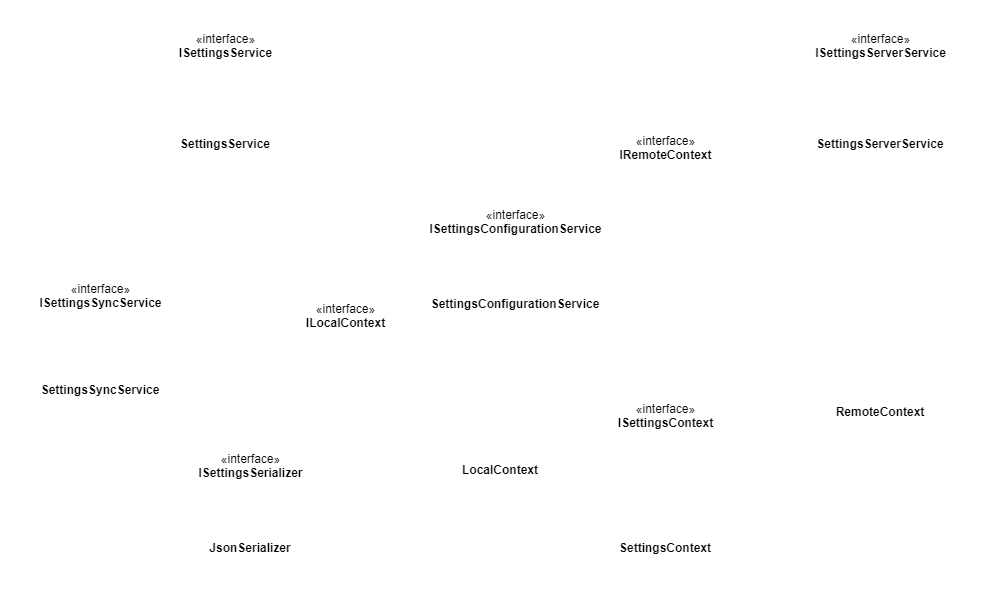
\includegraphics[scale=0.325]{../images/components transparent.png}
      \end{figure}
    \end{frame} 

    \subsection{Policy}
    \begin{frame}{Policy}
      \framesubtitle{Definizione ed utilizzo}
      \begin{block}{Definizione}
        Una \textbf{policy} è un comportamento che deve assumere il modulo nei confronti di determinati dati.
      \end{block}
      \begin{itemize}
        \item Definite attraverso programma apposito
        \item Utilizzate per definire i valori predefiniti
        \item Utilizzate per definire la mutabilità dei dati
        \item Utilizzare per definire le logiche di sincronizzazione
      \end{itemize}

    \end{frame}

    \subsection{Sincronizzazione}
    \begin{frame}{Sincronizzazione}
      \framesubtitle{Logiche di sincronizzazione}
      3 casi possibili durante la sincronizzazione:
      \begin{itemize}
        \item Valore remoto aggiornato e valore locale immutato
        \item Valore remoto immutato e valore locale aggiornato
        \item Entrambi i valori aggiornati
      \end{itemize}

      \begin{block}{Policy predefinita}
        La policy predefinita in caso di conflitto consiste nello scegliere il valore aggiornato più recentemente.\\
        Avviene invece una fusione in caso si tratti di liste.
      \end{block}

    \end{frame}

    \subsection{Integrazione}
    \begin{frame}{Integrazione}
      \begin{itemize}
        \item Integrazione avviene in fasi separate
        \item Focus sui "montaggi"
        \item Modifiche a modelli di dati già esistenti
      \end{itemize}
    \end{frame}

    \subsection{Conclusioni}
    \begin{frame}{Conclusioni}
      \textbf{Stato del progetto alla fine del tirocinio}
      \begin{itemize}
        \item Modulo completato
        \item Integrazione parziale perchè...
      \end{itemize}
      \textbf{Prospettive future}
      \begin{itemize}
        \item Supporto all'archiviazione su cloud
        \item Upgrade all'ultima versione di .NET
      \end{itemize}
    \end{frame}

    \begin{frame}{Conclusioni}
      \textbf{Grazie per l'attenzione.}
    \end{frame}

  \end{darkframes}
  
\end{document}
